\documentclass[12pt]{article}

\usepackage[utf8]{inputenc}
\usepackage{latexsym,amsfonts,amssymb,amsthm,amsmath}
\usepackage{float}

\setlength{\parindent}{0in}
\setlength{\oddsidemargin}{0in}
\setlength{\textwidth}{6.5in}
\setlength{\textheight}{8.8in}
\setlength{\topmargin}{0in}
\setlength{\headheight}{18pt}
\usepackage{graphicx}

\usepackage{hyperref}
\hypersetup{
    colorlinks=true,
    linkcolor=blue,
    filecolor=magenta,      
    urlcolor=cyan,
    pdftitle={Overleaf Example},
    pdfpagemode=FullScreen,
    }

\urlstyle{same}

\usepackage{caption}
\DeclareCaptionFormat{citation}{%
  \ifx\captioncitation\relax\relax\else
    \captioncitation\par
  \fi
  #1#2#3\par}
\newcommand*\setcaptioncitation[1]{\def\captioncitation{\textit{Source:}~#1}}
\let\captioncitation\relax
\captionsetup{format=citation,justification=centering}


\title{MATH1034OL1 Pre-Calculus Mathematics Notes from Sections 4.8, 3.3 (Monday)}
\author{Elijah Renner}

\begin{document}

\maketitle

\vspace{0.5in}

\tableofcontents

\section{Inverse Trigonometric Functions}

The three inverse trigonometric functions are \(\arccos\), \(\arcsin\), and \(\arctan\). These functions have the property\\

\[\arccos(x)=A\]
\[\cos(A)=x\]\\

In other words, \(\cos\) and \(\arccos\) are inverses of each other. They're helpful for determining an angle given its \(\sin, \cos,\) or \(\tan\) value.\\

When we're finding \(\arcsin(x)\), we restrict the range of \(\arcsin\) such that it remains a function (that is, there are no two outputs \(\arcsin(x)\) for one input \(x\)). We do this for all inverse trigonometric functions. Here are the restrictions:\\

\begin{figure}[H]
	\centering
	\includegraphics[scale=0.6]{arcf.gif}
	\caption{Credit: \url{https://www.mathnstuff.com/math/spoken/here/2class/330/arc.htm}}
\end{figure}

Problem: Find the Exact value of \(\sec\{\arctan[\sin(\arccos(\frac{-1}{2}))]\}\).\\

First, recall that \(\arccos(\frac{-1}{2})\) will be the angle whose cosine value is \(\frac{-1}{2}\). We know this angle is \(\frac{2\pi}{3}\) using the rules above.\\

Next, we determine that \(\sin(\frac{2\pi}{3})=\frac{\sqrt{3}}{2}\). This is where things get a little more complicated. \(\arctan(\frac{\sqrt{3}}{2})\) isn't an angle with reference angle \(30^{\circ}, 45^{\circ}, 60^{\circ}, 90^{\circ}\). This is fine because, when we zoom out, we're asked to find \(\sec(\arctan(\frac{\sqrt{3}}{2}))\). We know that the triangle formed by the angle \(\arctan(\frac{\sqrt{3}}{2})\) has \(\text{opp}=\sqrt{3}\) and \(\text{adj}=2\). We use the pythagorean theorem to find the hypotenuse:\\

\[(\sqrt{3})^2+2^2=c^2\]
\[\implies c=\sqrt{3+4}=\sqrt{7}\]\\

Hence, \(\text{hyp}=\sqrt{7}\). Even though the angle \(\arctan(\frac{\sqrt{3}}{2})\) doesn't form a special triangle, we can still find its \(\sec\) value using the sides of the triangle it forms:\\

\[\sec\left(\arctan\left(\frac{\sqrt{3}}{2}\right)\right)=\frac{\text{hyp}}{\text{adj}}=\frac{\sqrt{7}}{2}\]\\

Knowing this, \(\sec\{\arctan[\sin(\arccos(\frac{-1}{2}))]\}=\frac{\sqrt{7}}{2}\).

\section{Polynomial Long Division}

Polynomial division isn't easily explained in notes, but it's very important!. Here is my recommended resource for polynomial division:\\

\url{https://www.mathsisfun.com/algebra/polynomials-division-long.html}

\section{Remainder Theroem}

\begin{figure}[H]
	\centering
	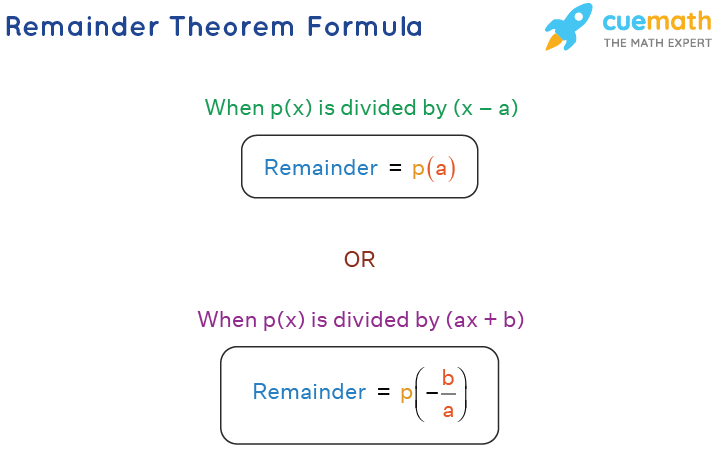
\includegraphics[scale=0.6]{rt.png}
	\caption{Credit: \url{https://www.cuemath.com/algebra/remainder-theorem/}}
\end{figure}


\section{Descarte's Rule of Signs}

\begin{figure}[H]
	\centering
	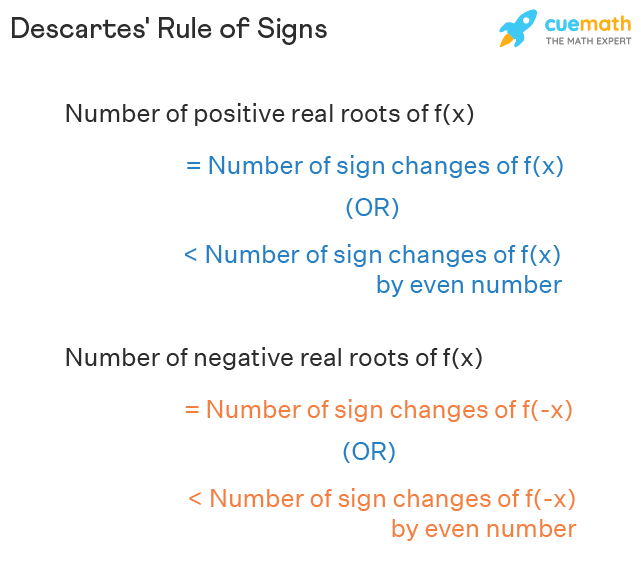
\includegraphics[scale=0.6]{drs.png}
	\caption{Credit: \url{https://www.cuemath.com/algebra/descartes-rule-of-signs/}}
\end{figure}

\begin{figure}[H]
	\centering
	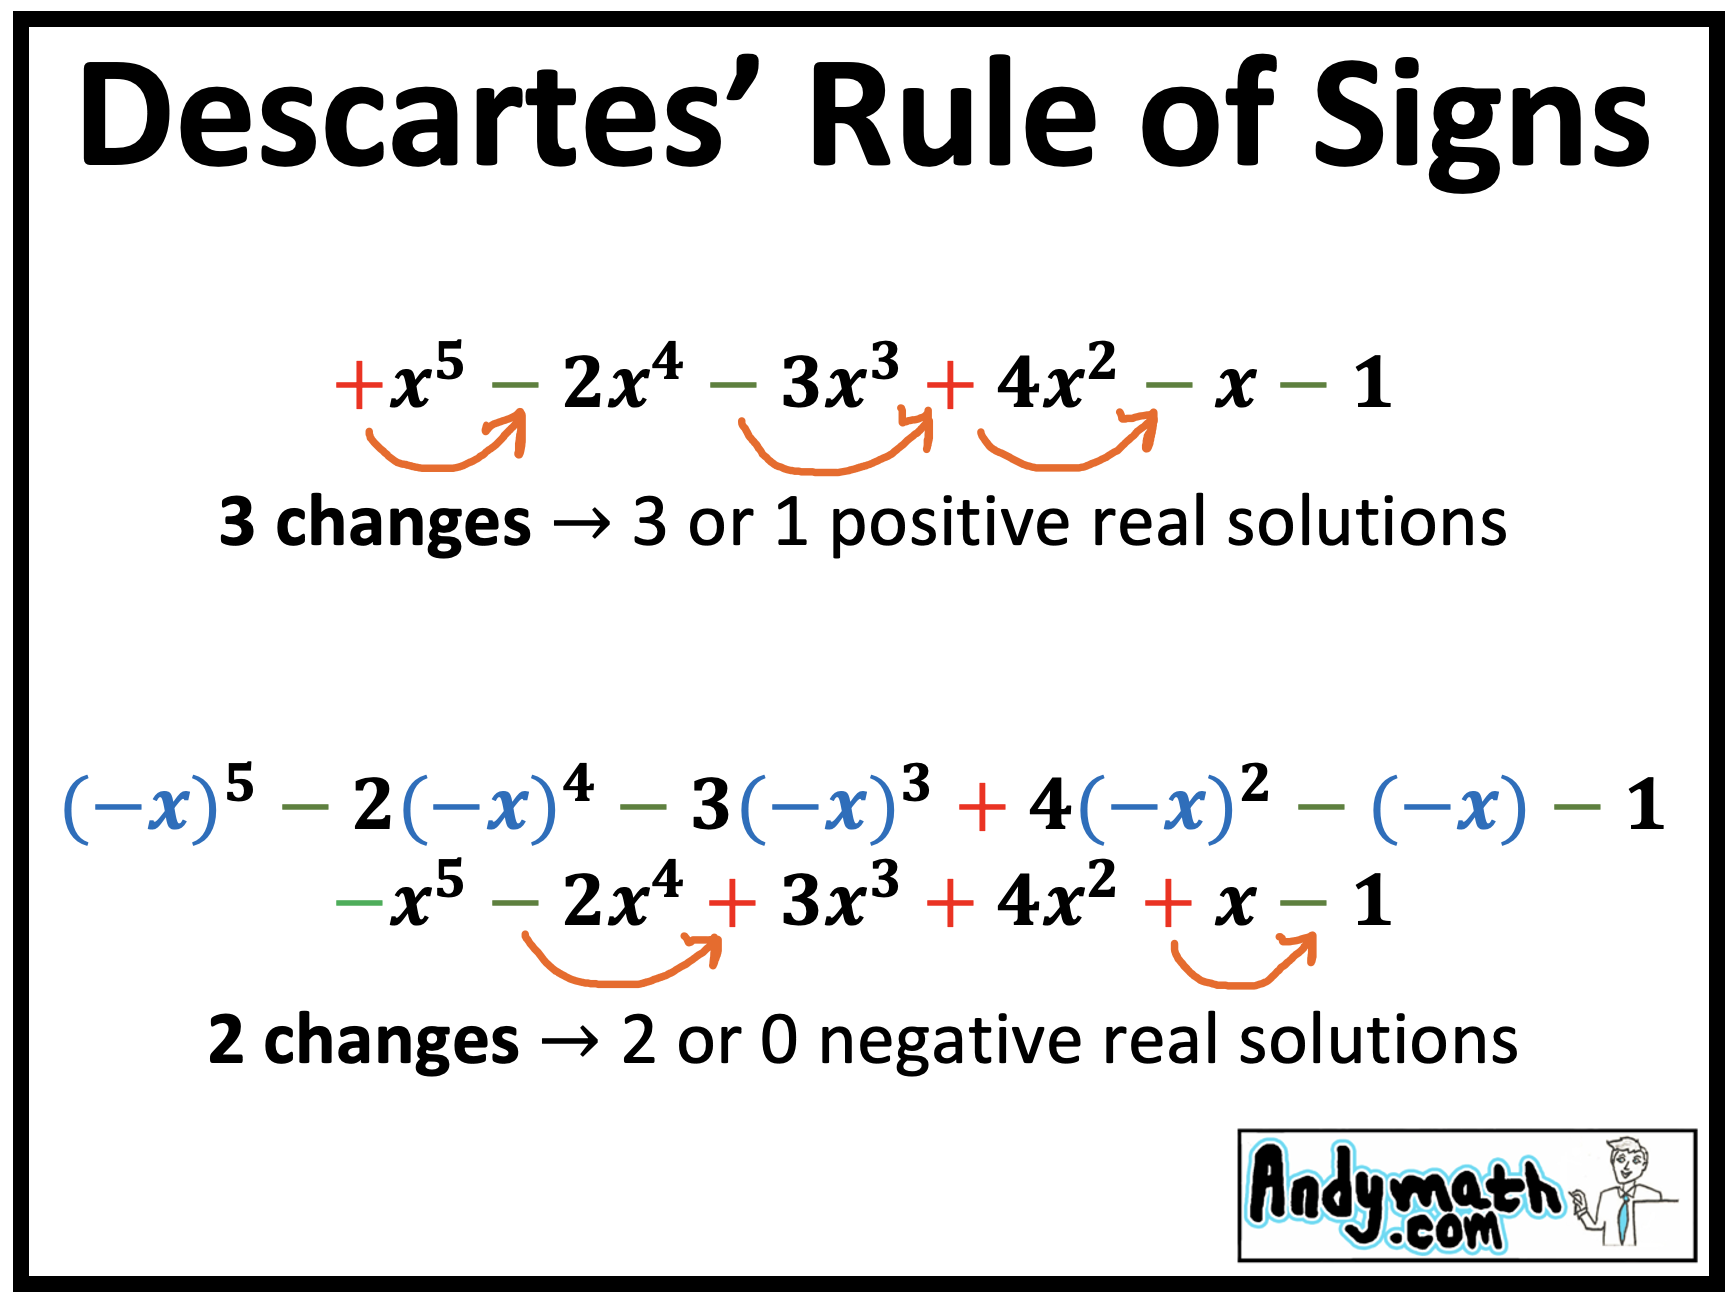
\includegraphics[scale=0.3]{drs2.png}
	\caption{Credit: \url{https://andymath.com/descartes-rule-of-signs/}}
\end{figure}

\end{document}
